\lecture{27}{11. December 2025}{Buckling of columns}

\section{Buckling of Columns}

\subsection{Critical Load}
A member must not only satisfy strength and deflection requirements, but it must also be stable -- This is particularly important if the member is long and slender and it supports compressive loading that becomes large enough to cause the members to suddenly deflect laterally or sideways.
These members are called \textit{columns}, and the lateral deflection that occurs is called \textit{buckling}.
Buckling can lead to sudden and dramatic failure of a mechanism, and as a result, attention must be given to the design of columns so they can safely support their intended loadings without buckling.

\begin{figure} [ht]
  \centering
  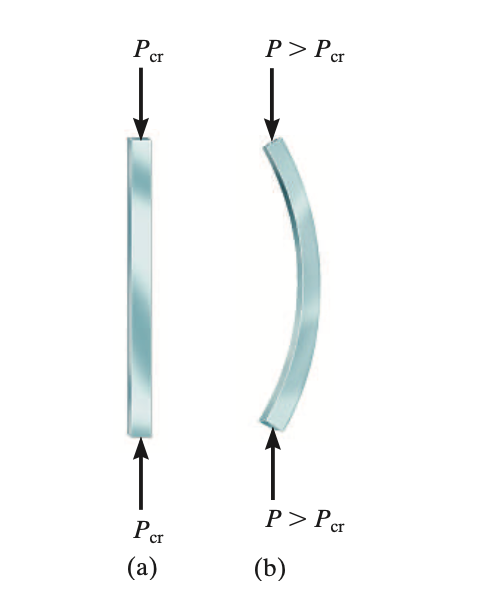
\includegraphics[width=0.4\linewidth]{./figures/f17_1a.png}
  \caption{Column on verge of buckling.}
  \label{fig:f17_1a}
\end{figure}

The maximum axial load a column can support on the verge of buckling is called the \textit{critical load}, $P_{\mathrm{cr}}$, shown on \Cref{fig:f17_1a}.
Any slight additional loading beyond this will cause the column to buckle and deflect laterally.

\begin{figure} [ht]
  \centering
  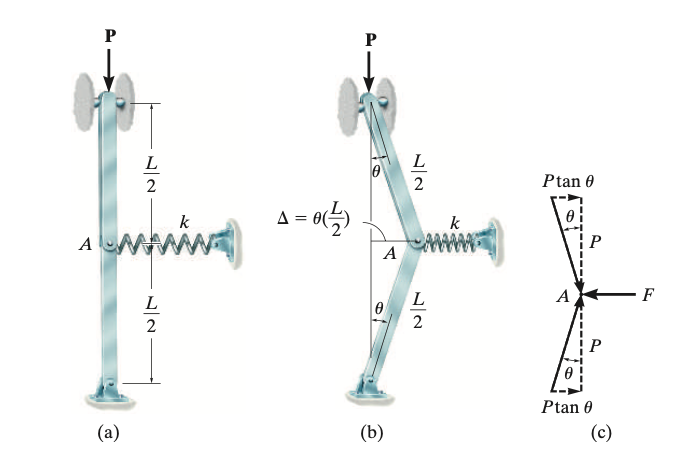
\includegraphics[width=0.75\linewidth]{./figures/f17_2a.png}
  \caption{Simplified model of buckling column.}
  \label{fig:f17_2a}
\end{figure}

We consider this instability as a two-bar mechanism consisting of rigid weightless bars that are pin-connected as shown on \Cref{fig:f17_2a}a.
When the bars are in the vertical position, the spring, having a stiffness $k$, is unstretched, and a \textit{small} vertical force $\Vec{P}$ is applied at the top of one of the bars.
To upset equilibrium, the pin at $A$ is displaced by a small amount $\Delta$, shown on \Cref{fig:f17_2}b.
As shown on the free-body diagram of the pin on \Cref{fig:f17_2}c, the sprinc will produce a restoring force $F = k \Delta$ in order to resist the two horizontal components $P_x = P \tan \theta$.
Since $\theta$ is small $\Delta \approx \theta L / 2$ and $\tan \theta \approx \theta$.
Thus the restoring spring force becomes $F = k \theta L / 2$ and the disturbing force is $2 P_x = 2 P \theta$.

If the restoring force is greater than the disturbing force, then, we can solve for $P$ which gives:
\begin{equation*}
  P < \frac{kL}{4} \qquad \text{Stable equilibrium}
.\end{equation*}
Or
\begin{equation*}
  P > \frac{kL}{4} \qquad \text{Unstable equilibrium}
.\end{equation*}

The critical load is right at
\begin{equation*}
  P_{\mathrm{cr}} = \frac{kL}{4}
.\end{equation*}
Since $P_{\mathrm{cr}}$ is independent of the small displacement $\theta$ of the bars, any slight disturbance given to the mechanism will not cause it to move further out of equilibrium, nor will it be restored to its original position.
Instead the bard will \textit{remain} in the deflected position.

These three different states of equilibrium are represented on \Cref{fig:f17_3a}.
The transition point where the load is equal to the critical value $P = P_{\mathrm{cr}}$ is called the \textit{bifurcation point}.
Here the bars will be in neutral equilibrium for any small value of $\theta$.


\begin{figure} [ht]
  \centering
  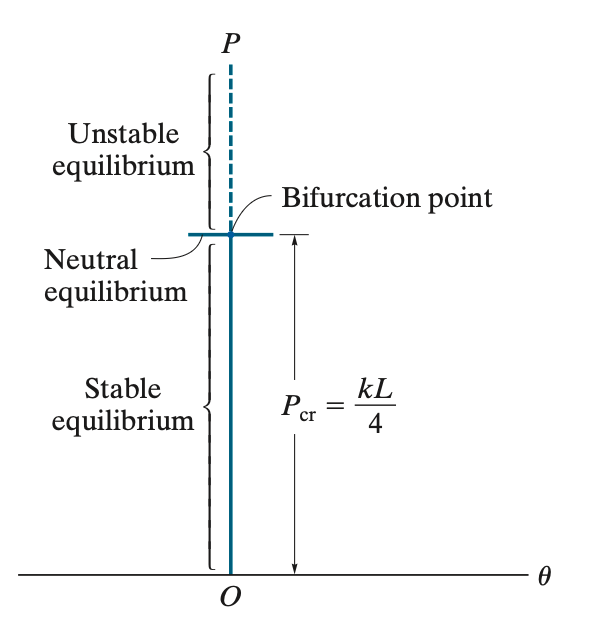
\includegraphics[width=0.4\linewidth]{./figures/f17_3a.png}
  \caption{Bifurcation point.}
  \label{fig:f17_3a}
\end{figure}

\subsection{Ideal Column with Pin Supports}
We consider a pin and roller supported column as shown on \Cref{fig:f17_4a}, which we will term an \textit{ideal column}, meaning it is made of a homogeneous linear elastic material and is perfectly straight before loading.
Here, the load is applied through the centroid of the section.

\begin{figure} [ht]
  \centering
  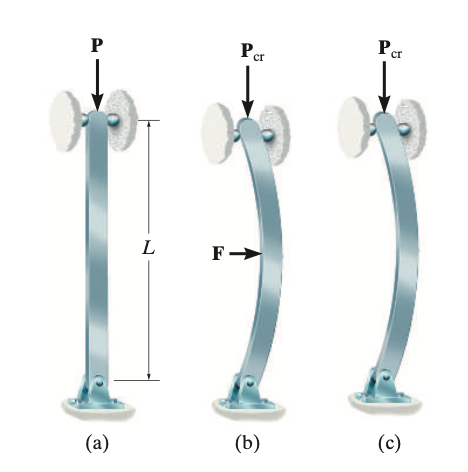
\includegraphics[width=0.5\linewidth]{./figures/f17_4a.png}
  \caption{Column with pin and roller supports.}
  \label{fig:f17_4a}
\end{figure}

The tendency for a column to remain stable or become unstable when subjected to an axial load depends upon its ability to resist bending.
Hence, in order to determine the critical load and the buckled shape of the column, we use
\begin{equation*}
  EI \frac{\mathrm{d}^2 v}{\mathrm{d}x^2} = M
.\end{equation*}

\begin{figure} [ht]
  \centering
  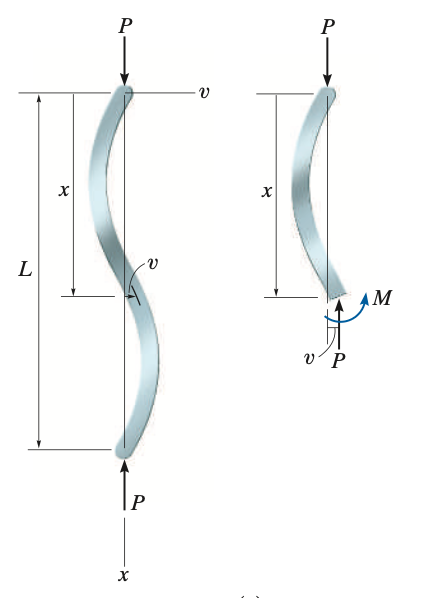
\includegraphics[width=0.5\linewidth]{./figures/f17_5.png}
  \caption{Free body diagram of buckled column.}
  \label{fig:f17_5}
\end{figure}

A free-body diagram of a segment of the column in the deflected position is shown on \Cref{fig:f17_5}.
Moment equilibrium requires
\begin{equation*}
  M = - Pv
\end{equation*}
so
\begin{align*}
  EI \frac{\mathrm{d}^2 v}{\mathrm{d}x^2} &= -Pv \\
  \frac{\mathrm{d}^2 v}{\mathrm{d}x^2} + \left( \frac{P}{EI} \right) v &= 0
.\end{align*}
The general solution to this homogeneous, second-order linear differential equation with constant coefficients is
\begin{equation*}
  v = C_1 \sin \left( \sqrt{\frac{P}{EI}} x  \right) + C_2 \cos \left( \sqrt{\frac{P}{EI}} x \right)
.\end{equation*}
Since $v = 0$ at $x = 0$, $C_2 = 0$ and since $v = 0$ at $x = L$, then
\begin{equation*}
  C_1 \sin \left( \sqrt{\frac{P}{EI}}L \right) = 0
.\end{equation*}
This requires
\begin{equation*}
  \sin \left( \sqrt{\frac{P}{EI}}L  \right)= 0
\end{equation*}
which is satisfied if
\begin{equation*}
  \sqrt{\frac{P}{EI}} L = n \pi
\end{equation*}
or
\begin{equation*}
  P = \frac{n^2 \pi^2 EI}{L^2}, \quad n = 1,2,3,\ldots 
.\end{equation*}

The smallest value of $P$ is for $n = 1$ ($n$ is the number of curves in the deflected shape of the column), so the critical load is:
\begin{equation*}
  P_{\mathrm{cr}} = \frac{\pi^2 EI}{L^2}
\end{equation*}
which is also referred to as the \textit{Euler load}.
The corresponding buckled shape is
\begin{equation*}
  v = C_1 \sin \frac{\pi x}{L}
.\end{equation*}
The constant $C_1$ represents the maximum deflection $v_{\mathrm{max}}$ which occurs at the midpoint.

I.e.
\begin{equation*}
  P_{\mathrm{cr}} = \frac{\pi^2 EI}{L^2}
\end{equation*}
where
\begin{itemize}
  \item $P_{cr}$ is the critical or maximum axial load on the column before it begins to buckle.
  \item $E$ is the modulus of elasticity
  \item $I$ is the \textit{least} moment of inertia for the column's cross-sectional area
  \item $L$ is the unsupported length of the column
\end{itemize}

For design purposes, this can be written in terms of stress using $I = A r^2$, where $A$ is the cross-sectional area and $r$ is the \textit{radius of gyration} of the cross sectional area.
We have,
\begin{align*}
  \sigma_{\mathrm{cr}} = \frac{\pi^2 E}{\left( \frac{L}{r} \right)^2}
\end{align*}
Where
\begin{itemize}
  \item $\sigma_{\mathrm{cr}}$ is the critical stress
  \item $E$ is the modulus of elasticity
  \item $L$ is the unsupported length of the column
  \item $r$ is the smallest radius of gyration of the column given by $r = \sqrt{I / a}$
\end{itemize}


\subsection{Columns Having Various Types of Supports}
The Euler load above was derived for column that is pin connected.
Columns can, however, also be supported differently.

\paragraph{Effective Length}
To use Euler's formula, for columns having different types of supports, we will modify the column length $L$ to represent the distance between the points of zero moment on the column.
This distance is called the column's effective length $L_e$.
For a pin-ended column $L_3 = L$ as shown on \Cref{fig:f17_10}a.
For the fixed-end and free-ended column the effective length is $L_3 = 2L$ as shown on \Cref{fig:f17_10}b.
Other examples are shown on \Cref{fig:f17_10}c and \Cref{fig:f17_10}d.

\begin{figure} [ht]
  \centering
  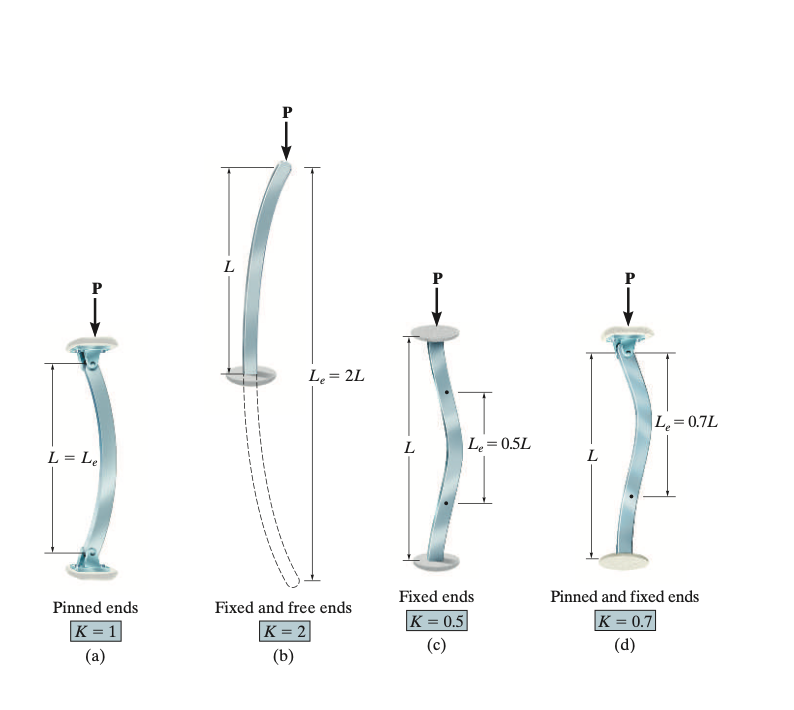
\includegraphics[width=0.8\linewidth]{./figures/f17_10.png}
  \caption{Effective lengths of columns fixed in different ways.}
  \label{fig:f17_10}
\end{figure}

Rather than specifying the column's effective length, many design codes provide column formulas that employ a dimensionless coefficient $K$ called the \textit{effective length factor}, defined from
\begin{equation*}
  L_e = K L
.\end{equation*}
Based on this generality, we can write Euler's formula as
\begin{equation*}
  P_{\mathrm{cr}} = \frac{\pi^2 EI}{\left( KL \right)^2}
\end{equation*}
or
\begin{equation*}
  \sigma_{\mathrm{cr}} = \frac{\pi^2 E}{\left( \frac{KL}{r} \right)^2}
.\end{equation*}

